\documentclass{beamer}
\usetheme{Pittsburgh}
\beamertemplatenavigationsymbolsempty


\usepackage{amsmath}
\usepackage{amssymb}
\usepackage{bm} % For bold math symbols
\usepackage{graphicx}
\usepackage{tikz}



\usepackage{subfig} % Changed from subfigure (deprecated)
\usepackage{multirow}
\usepackage{multicol}
\usepackage{color}
\usepackage{url}
\usepackage{hyperref}
\usepackage{listings}
\usepackage[noend]{algorithm}
\usepackage{physics} 
% add image path
\graphicspath{{../Images/}}






\DeclareMathOperator{\argmin}{argmin}
\DeclareMathOperator{\argmax}{argmax}






\title{Weekly Updates\\
\tiny{Wednesday, 15/05/2025}}
\author{Andrea Bonifacio}
\date{}

\begin{document}

\begin{frame}
\titlepage
\end{frame}

\begin{frame}{Recap: Project Goals \& Status}
    \begin{itemize}
        \item Here's a brief recap of what we did up until now.
        \item In the first half of this project we started implementing a method that uses neural networks to compute the nonlinear correction of the displacement field.
        \item The idea was interesting, with some already existing methods in the field of CFD, but at some point we realized that the method was not easily applicable to our case, especially for the dynamic case.
        \item We decided to explore a different method, which is based on the idea of using a neural network to ``correct'' the linear modes of a structure.
    \end{itemize}
\end{frame}

\begin{frame}{Overview of Work Done}
    \begin{itemize}
        \item While the first part of the project was not very successful, helped us a lot to understand the problem and create the necessary tools to implement the new method.
        \item We learned the limitations and strengths of the numerical solver we are using (SOFA).
        \item The main idea is still to somehow correct a displacement field, but this new method is based on a self-supervised approach, removing the need for a dataset.
    \end{itemize}
\end{frame}



\begin{frame}{Neural Modes Paper - Key Ideas}
    \begin{itemize}
        \item The paper wants to extend the concept of linear modes to ``neural modes''.
        \item The idea is to compute a non-linear correction of the displacement field, by having the network minimize the energy of the system.
        \item Once the network has been trained and learned the non-linear modes for any modal coordinate in the subspace, it can be extended to dynamics by using a finite difference scheme.
    \end{itemize}
\end{frame}






\begin{frame}{Mechanical Model: Neo-Hookean Hyperelasticity}
    \begin{itemize}
        \item \textbf{Deformation Gradient:}
        \begin{equation*}
            \bm{F} = \frac{\partial \bm{x}}{\partial \bm{X}} = \bm{I} + \nabla_X \bm{u}
        \end{equation*}
        \item \textbf{Neo-Hookean Strain-Energy Density Function \(\Psi\):}
        \begin{equation*}
            \Psi(\bm{F}) = \frac{\mu}{2} (I_C - 3 - 2\ln(J)) + \frac{\lambda}{4} (J^2 - 1 - 2\ln(J))
        \end{equation*}
        \item \(J = \det(\bm{F})\), \(\mu\) (shear modulus), \(\lambda\) (Lamé's first parameter).
        \item Material parameters related to Young's modulus \(E\) and Poisson's ratio \(\nu\).
    \end{itemize}
\end{frame}


\begin{frame}{Linear Modal Analysis: Motivation}
    \begin{itemize}
        \item Simulating deformations in real-time is computationally challenging.
        \item \textbf{Modal Analysis:} Accelerates simulations by approximating complex deformations as a combination of dominant vibration patterns (modes).
        \item Reduces dimensionality by focusing on low-frequency modes.
        \item Enables faster simulations while maintaining reasonable accuracy for certain regimes.
    \end{itemize}
\end{frame}

\begin{frame}{Linear Modal Analysis: Core Steps}
    \begin{enumerate}
        \item \textbf{Linearize the System:}
        \begin{itemize}
            \item Linearize governing equations around undeformed state (\(\bm{u}=\bm{0}\)).
            \item Results in constant stiffness matrix \(\bm{K}\) and mass matrix \(\bm{M}\).
        \end{itemize}
        \item \textbf{Solve Generalized Eigenvalue Problem:}
        \begin{equation*}
            \bm{K} \bm{\phi}_i = \omega_i^2 \bm{M} \bm{\phi}_i
        \end{equation*}
        \begin{itemize}
            \item \(\omega_i^2\): Eigenvalues (squared natural frequencies).
            \item \(\bm{\phi}_i\): Eigenvectors (mode shapes).
        \end{itemize}
    \end{enumerate}
\end{frame}

\begin{frame}{Linear Modal Analysis: Modal Decomposition \& Limitations}
    \begin{itemize}
        \item \textbf{Modal Decomposition (Reduced Basis):}
        \begin{itemize}
            \item Select first \(m\) modes (lowest frequencies).
            \item Approximate displacement:
            \begin{equation*}
                \bm{u}(\bm{X},t) \approx \sum_{i=1}^{m} q_i(t) \bm{\phi}_i(\bm{X})
            \end{equation*}
            \item \(q_i(t)\): Time-varying modal coordinates.
        \end{itemize}
        \item \textbf{Fundamental Limitation:}
        \begin{itemize}
            \item Initial linearization holds well only for \textbf{small deformations}.
            \item Breaks down for large, nonlinear deformations (e.g., hyperelastic materials).
            \item Constant \(\bm{K}\) doesn't capture nonlinear material resistance.
        \end{itemize}
        \item \textbf{Motivation for Neural Modes:} Overcome these limitations by incorporating nonlinear effects.
    \end{itemize}
\end{frame}


\begin{frame}{Neural Modes Architecture}
    \begin{itemize}
        \item \textbf{Goal:} Learn nonlinear corrections to linear deformation modes for Neo-Hookean materials.
        \item \textbf{Input:} Modal coordinate vector \( \bm{z} \in \mathbb{R}^m \).
        \item \textbf{Core:} Deep residual neural network.
        \begin{itemize}
            \item Several residual blocks (fully connected layers + Leaky ReLU + skip connection).
        \end{itemize}
        \item \textbf{Output:} Nonlinear correction to displacement field \( \bm{y} \in \mathbb{R}^n \).
    \end{itemize}
    \begin{center}
        
        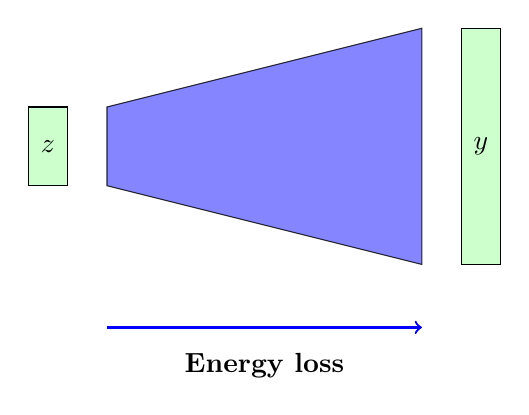
\begin{tikzpicture}
            % Modal coordinate (z)
            \draw[fill=green!20] (-3, 1) rectangle (-2.5,2);
            \node at (-2.75, 1.5) {$z$}; % Label inside the rectangle
            
            % Displacement (u)
            \draw[fill=green!20] (2.5,0) rectangle (3,3);
            \node at (2.75, 1.5) {$y$}; % Label inside the rectangle
            
            % Energy loss transition
            \draw[fill=blue!60,opacity=0.8] (-2,1) -- (2,-0) -- (2,3) -- (-2,2) -- cycle;
            \node[below] at (0,-1) {\textbf{Energy loss}};
            
            % Energy loss arrow
            \draw[thick,blue,->] (-2,-0.8) -- (2,-0.8);
        
        \end{tikzpicture}
\end{center}

\end{frame}

\begin{frame}{Training Neural Modes: Physics-Informed Loss}
    \begin{itemize}
        \item \textbf{Total Loss:} Weighted sum of:
        \begin{enumerate}
            \item \textbf{Energy Loss:} Minimize internal strain energy \(E(\bm{X} + \bm{l} + \bm{y})\).
            \begin{itemize}
                \item \(\bm{l}\): linear displacement from \(\bm{z}\).
                \item \(\bm{y}\): nonlinear correction from NN.
            \end{itemize}
            \item \textbf{Orthogonality Loss:} Ensure correction \(\bm{y}\) is orthogonal to linear modes: \(\bm{y}^T \bm{l} = 0\).
            \item \textbf{Boundary Condition Penalty:} Enforce displacement BCs.
        \end{enumerate}
        \begin{equation*}
            \text{Loss} = E(\bm{X} + \bm{l} + \bm{y}) + \lambda_1 (\bm{y}^T \bm{l})^2 + \lambda_2 \text{BC Penalty}
        \end{equation*}
        \item \textbf{Zero Correction at Origin:} Ensured by bias-free NN architecture (output is zero if \(\bm{z}=\bm{0}\)).
    \end{itemize}
\end{frame}



\begin{frame}{Dynamic Simulation with Neural Modes}
    \begin{itemize}
        \item At each time step \(n+1\), solve for modal coordinates \(\bm{z}_{n+1}\):
        \begin{equation*}
            \bm{z}_{n+1} = \underset{\bm{z}}{\argmin} \frac{1}{2h^2} \|\bm{n}(\bm{z}) - 2\bm{u}_n + \bm{u}_{n-1}\|_{\bm{M}}^2 + E(\bm{n}(\bm{z}))
        \end{equation*}
        \begin{itemize}
            \item \(\bm{n}(\bm{z}) = \bm{l}(\bm{z}) + \bm{y}(\bm{z})\): Full displacement (linear + NN correction).
            \item \(h\): time step, \(\bm{M}\): mass matrix.
            \item Solved using L-BFGS-B.
        \end{itemize}
        \item  Current formulation doesn't explicitly account for external forces.
        \begin{itemize}
            \item Network minimizes internal energy.
            \item May affect accuracy for large deformations or complex external loads.
        \end{itemize}
    \end{itemize}
\end{frame}

\begin{frame}{Neural Modes Paper - Our Implementation}
    \begin{itemize}
        \item We developed a fully differentiable energy calculator for both StVenant-Kirchhoff and Neo-Hookean materials, completely written in PyTorch, that helps with the training speed.
        \item Also the eigenvalue problem is solved directly using SOFA, which enables faster prototyping and testing.
        \item We observed good results for small deformations, but the energy from linear modes tend to explode for larger deformations.
    \end{itemize}
\end{frame}

\begin{frame}
    \frametitle{Our Results}
    \begin{centering}
        \includegraphics[width=0.8\textwidth]{Images/results_no_train.png}
        \captionof{figure}{Energies for the nonlinear elastic beam, the linear elastic beam, the linear modes, and the neural modes.}
    
    \end{centering}
\end{frame}

\begin{frame}{Determining the Number of Modes (\(m\))}
    \begin{itemize}
        \item The choice of \(m\) (number of linear modes to form the subspace) is crucial.
        \begin{itemize}
            \item Too few: May not capture enough of the object's deformation behavior, even with NN correction.
            \item Too many: Increases the dimensionality of \(\bm{z}\), potentially making NN training harder and dynamic optimization slower.
        \end{itemize}
        \item \textbf{Empirical Approach:}
        \begin{itemize}
            \item Start with a reasonable number (e.g., 10-20).
            \item Evaluate reconstruction error of linear modes for target deformations.
            \item For our beam examples, \(m \approx 10\) modes often provided a good balance.
        \end{itemize}
    \end{itemize}
\end{frame}

\begin{frame}
    \frametitle{Choosing the Number of Modes (\(m\))}
    \begin{centering}
        \includegraphics[width=0.8\textwidth]{Images/mse_10_modes.png}
        \captionof{figure}{Mean Squared Error (MSE) of the linear modes for 10 modes.}
    \end{centering}

\end{frame}

\begin{frame}{Optimal Sampling of Modal Coordinates (\(\bm{z}\))}
    \begin{itemize}
        \item During NN training, we need to sample modal coordinates \(\bm{z}\) to generate linear displacements \(\bm{l}(\bm{z})\) for the loss function.
        \item We use a uniform distribution to sample \(\bm{z}\) values.

        \item \textbf{Question:} Is uniform sampling the best approach? Randomly sampled \(\bm{z}\) values might create unnatural or unrealistic deformations. Also, lower frequency modes contribute more significantly to the overall deformation.
        \item Maybe adaptive sampling or importance sampling based on observed errors or energy gradients during training.
    \end{itemize}
\end{frame}

\begin{frame}{Issues: Minimizing Only Internal Energy}
    \begin{itemize}
        \item The original "Neural Modes" paper proposes minimizing only the internal elastic energy \(E(\bm{n}(\bm{z}))\) during the dynamic step.
        \item Is this sufficient when significant external forces or prescribed displacements are present?
        \begin{itemize}
            \item The system should find a state that balances internal forces with external influences.
            \item Minimizing only internal energy might lead to unrealistic behavior if external work is not considered.
            \item For example, a constant external force should lead to a static equilibrium where internal and external forces balance, not necessarily the absolute minimum internal energy.
        \end{itemize}
    \end{itemize}
\end{frame}




\begin{frame}
    \frametitle{Concluding Questions and Future Directions}
    \begin{itemize}
        \item What should we address in the remaining time?
        \item Are neural modes just a nonlinear version of the linear modes (i.e. they work well for small deformations)?
        \item Is the work done so far good, or there is something we could explore more to wrap up the project?
    \end{itemize}
\end{frame}
\begin{frame}
    \begin{center}
        \color{blue} \Huge{Questions?}
    \end{center}

\end{frame}
\end{document}

